\section{Overview: High-level components and their interaction}
The system is organized following the three tiers architecture. This aims to decouple logical layers in order to gurantee an horizontal scalability and an high fault tolerance.
Graphically it's shown in the figure \ref{3-tier}.
\par

\textbf{Presentation layer}. It's the front-end layer which consists of the user interface. We have two types of user interface, depending on his functionality: 
\begin{itemize}
\item \textbf{CLup}: It's the mobile application used by users who have a smartphone. They can manage their booking by themselves;
\item \textbf{CLup Operator}: It's the desktop application used by receptionists that act as an intermediary to manage booking of users that have only a mobilephone.
\end{itemize}

\textbf{Application layer}. It deals with the model of the system, by containing the business logic of the application. In our system it consists in a remote server to which mobile and desktop applications have to connect due to manage any booking.

\textbf{Data layer}. It's composed by a data storage system. It includes: 


\begin{itemize}
\item User sensitive data asked during the registration process;
\item Information about user's grocery shopping;
\end{itemize}

\begin{figure}[H]
  \label{3tiers}
  \centering
  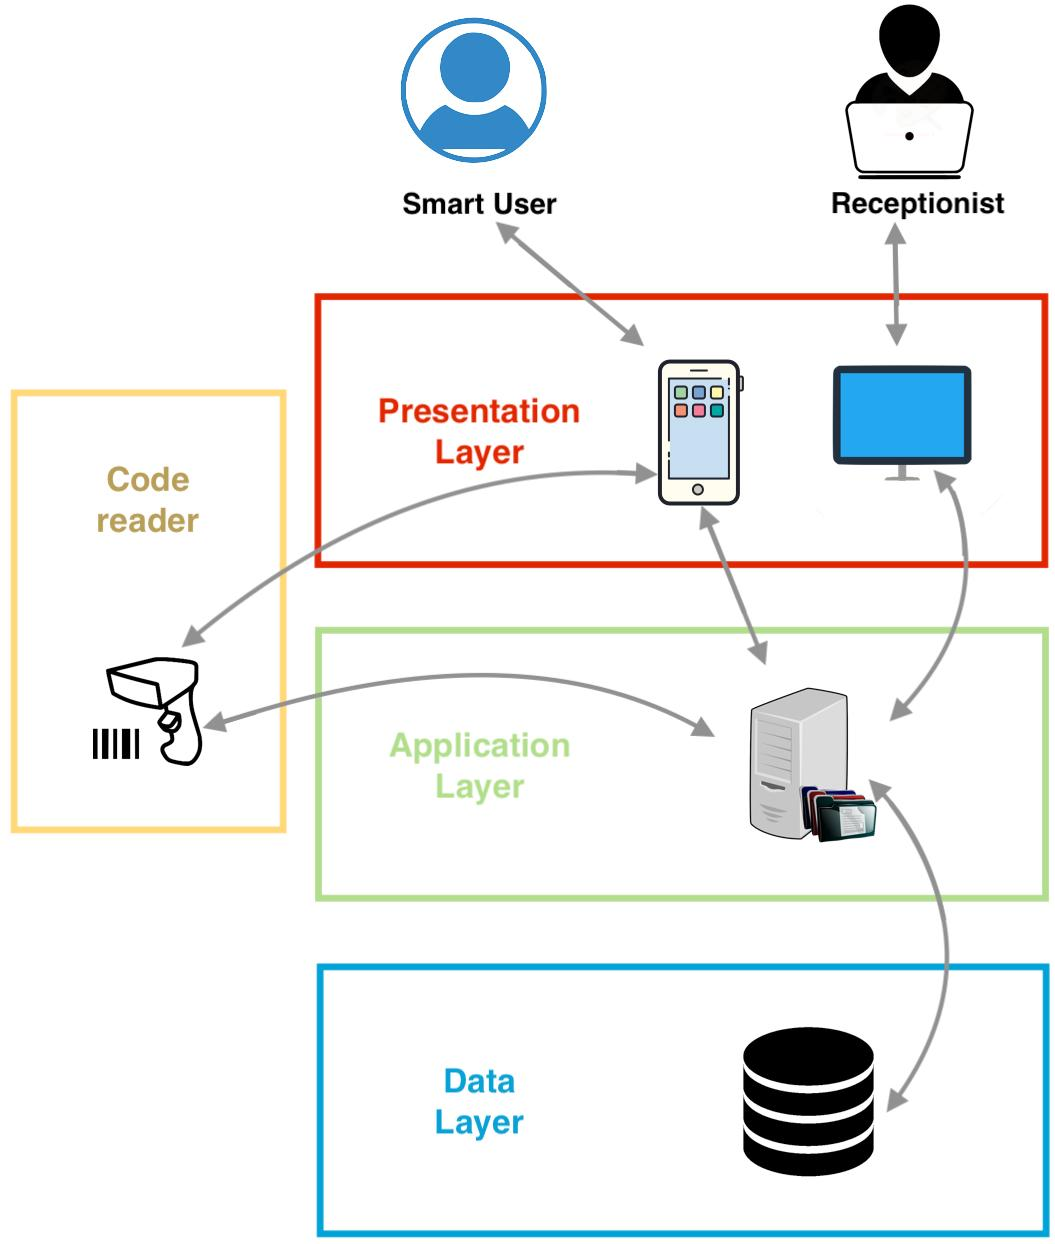
\includegraphics[scale=0.30]{diagrams/3_tiers.jpeg}
  \caption{Three tiers architecture of the system}
  \label{3-tier}

\end{figure}


\section{Component view}



In this section we describe the architecure with respect to its components and how they are wired together to form our system. 
Indeed, communication between Server and Clients is ensured by appropriate components which are called \textbf{Network Manager}. \par 
By an high-level point of view (figure \ref{fig:highlevel}) the main subsysystems correspond almost to the 3 layers in the 3 tiers architecture, with the addition of the \textbf{Market's subsystem}. \\ \\
The last one includes the \textbf{QRCode reader}, which has different functionality:
\begin{itemize}
\item It checks if QRCode at the entrance/exit is valid. If it's valid it will submit it. In addition a manual insertion of the QRCode is provided, due to allows Mobile Users to insert his code sent by SMS;
\item It controls the \textbf{Shop door}. When a QRCode is submitted, the reader allows users to enter by opening it;
\end{itemize}


\begin{figure}[H]
  \centering
  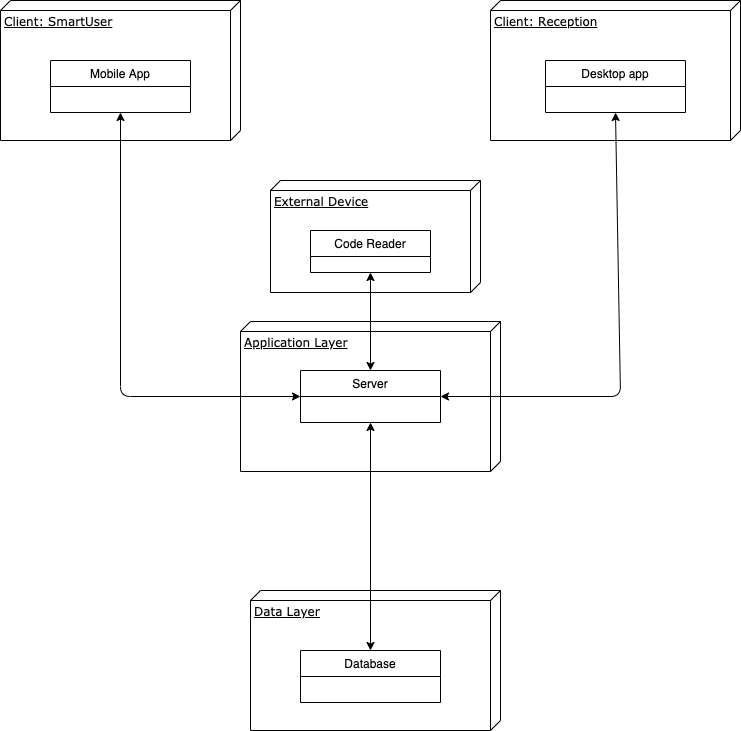
\includegraphics[scale=0.25]{diagrams/h_level.png}
  \caption{High-Level component diagram}
    \label{fig:highlevel}

\end{figure}



It follows a detailed description of the other significant components (figure       \ref{component_diagram}
)
\subsection{Application layer}
It's the core of our system. It's composed by:
\begin{itemize}
\item \textbf{Controller}: In our model this is th core ofour business logic. It deals with the stochastic time estimations to control the flux of users inside and outside the market. Moreover it uses interfaces provided from the other components linked to it;
\item \textbf{Auth User and Auth Reception}: these components grants respectively the access of users and receptionist by verifying their credential. In particular they are also accountable for users' registration;
\item \textbf{Visit Schedule and Reservation Queue}: they manage respectevely Visit and Reservation requests of Users and Receptionists. In addition they provides QRCodes;
\item \textbf{Notification Manager}: it's the component necessary to notify users about their turn in the queue. Furthermore, it responsible for sending SMS to user with mobilephone through an \textit{SMS Gateway};
\end{itemize}


\subsection{Client's layers: CLup and CLup Operator}
Each one of them is composed by components in a similar way, even if they have different functionalities.
Both they've got, as we can see in the figure 2.3:
\begin{itemize} 
\item \textbf{GUI component}: it provides the graphical interface in which User and Receptionist can interact with the system;
\item \textbf{Network Manager}: it's used to interact with the application server by sending or receiving informations; 
\end{itemize}


CLup is composed also by a \textbf{Request Handler} which exposes methods to User to handle any request or action needed. Then, it interacts with the Network Manager to send request to the Server. \par
Instead, CLup Operator has the \textbf{Booking Manager}, which is a similar component to the previous one but with more functionalities. In particular it handles any booking of mobile users and their sensitive information. So it's allowed by application server to query all users' sensitive data with higher privileges than CLup. \par




\begin{figure}[H]
  \centering
  \makebox[\linewidth]{
  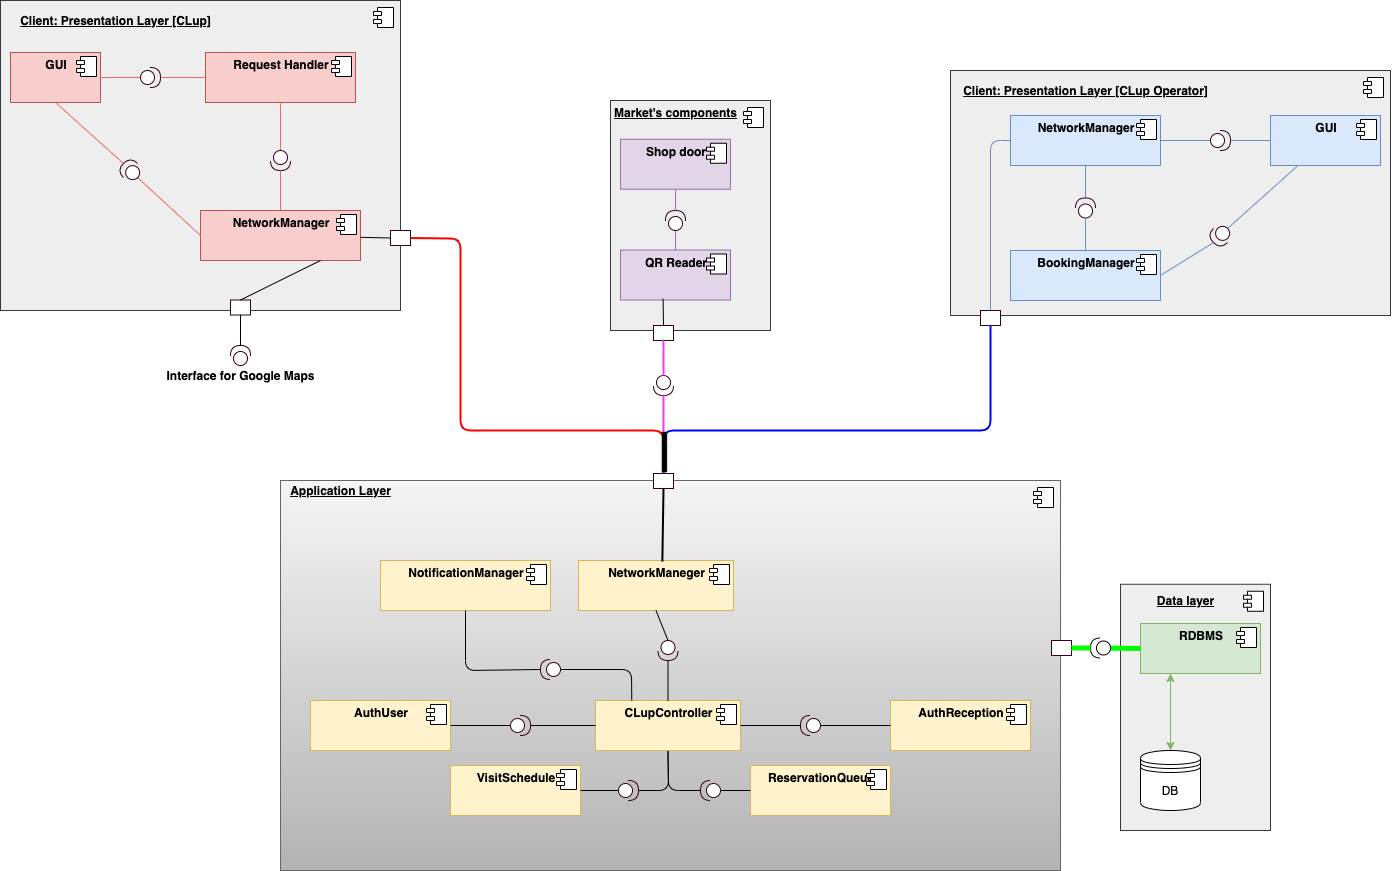
\includegraphics[scale=0.45]{diagrams/component_diagram.png}}
    \caption{Component Diagram}
      \label{component_diagram}

\end{figure}



\subsection{Data Layer}

In our architecture the data layer is composed by a relational DB needed to store informations about users and their dynamics in the market. 

In particular it should be connected to the server placed in the application layer. To reach the goal we plan to adopt a \textbf{RDBMS} in order to deal with a relational database. Indeed, it ensures consistency of data due to the \textit{ACID} properties.

In addition, it can process a large amount of data, which is suitable for our application. 

Besides, due to a better efficiency, RDBMS provides \textit{horizontal fragmentation}. It allows to fragment entities of our model with respect to each different market. This is why tuples regarding different markets will never be queryied together. The only which won't be fragmented is the Market entity. 

Moreover, it includes a software program which is designed to capture request over a network of the application server. From this each user and receptionist in fact could retrieve informations needed through SQL Query by connecting to it.  


An other important aspect is the security of the data due to mitigate any risks of violation. In order to do that we limit its access exclusively only to the application server. Communication between them will be also encrypted and accounts' passwords will be hashed.




\section{Deployment view}


\begin{figure}[H]
  \centering
  \makebox[\linewidth]{
  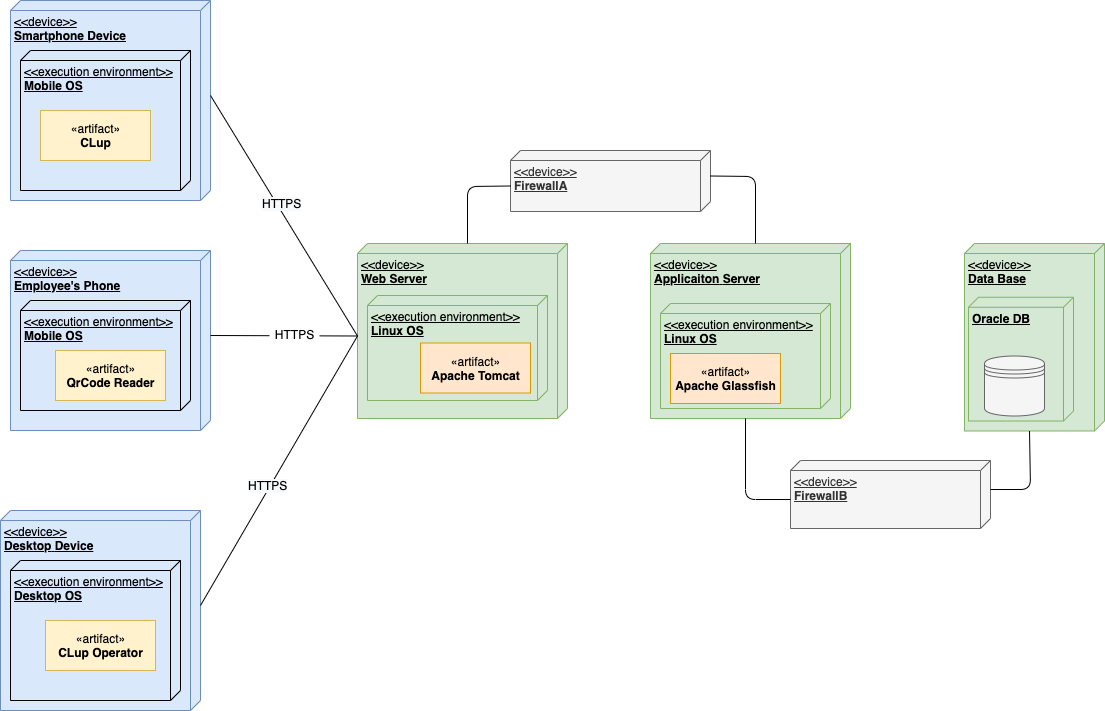
\includegraphics[scale=0.38]{diagrams/deployment.png}}
    \caption{Deployment Diagram}
      \label{fig:deployment}
\end{figure}



In this section we'll explain the structure of our run-time system and the interaction between the hardware and the software parts. This is shown in the deployment diagram in the figure \ref{fig:deployment}. \bigskip

For the client's side, CLup and CLup Operator will be hosted respectevely on a mobile and desktop device. Softwares will be designed both following a cross-platform development. 
We choose cross-platform to ensure an easier and quicker implementation; moreover it includes a better uniformity and maintenability.   
The main OSs choosen are respectevely iOS and Android for CLup and macOS and Windows for CLup Operator.\\
In addition is provided a third device used by a generic employee of the market which, interfaced with a QRCode scanner, sends to the server any request for entering or leaving  the market. \pagebreak

Instead, the server is organized as well following a \textbf{3 Tier Server Architecture}. Each tier is composed by:

\begin{enumerate}
\item \textbf{Web Server}: it's the node to which every clients connect. It handles each request from the clients connecting by HTTPS and is built using \textbf{Apache Tomcat}. \\
  %which can provide a web server. 
This, supported by Apache Software Foundation, a nonprofit corporation, is an open source software which is lightweight and suitable for our web server;
\item \textbf{Application Server}: this node hosts the core of our business logic. We set \textbf{Apache Glassfish} which is leading of the Java EE standard to run servlets. Compared to Tomcat, is a full-blown Java EE application server, because it includes more features. Indeed it provides backup and recovery services due to a better availability a reliability;

\item \textbf{Data Base}: this machine contains each data of our system. In fact it's composed by a \textbf{RDBMS} in order to store and retrieve data. Besides, we choose \textbf{Oracle DB} from Oracle Corporation as management system on it. We choose it because of its high performances, which are necessary to process data quickly. \\
In particular it can handles large volume of data since it have to manage a many users' requests simultaneously;
\end{enumerate}
\bigskip
Each tier is divided from the others with \textbf{2 Firewalls} which aim to filter any incoming and outgoing network traffic.
In particular:

\begin{itemize}

\item \textbf{FirewallA}: it filters traffic coming from the WS to AS. It allows requests from receptionist, logged user and employees' devices. This is due to mantaining the application server's integrity;

\item \textbf{FirewallB}: this protects the DB by filtering any packets, except for the application server. In this way we gurantee an high security against any data violation; 
\end{itemize}

\bigskip
\bigskip
\bigskip
\bigskip

\section{Runtime view}
In this section it will be illustrated the main runtime procedures of our system. We describe these by using Sequence Diagram in order to formalize how our components work together and in which order are used.

\pagebreak


\subsection{Login and registration}

Both processes start from the user's device where a request is elaborated by the \textit{Request Handler}. After the request passes to the Server's side where either login or registration is processed by \textit{Auth User}. Then, it established, by accessing to the \textit{RDBMS}, if the request can be validated or not. A return message was sent to the users for a success or failure operation. \\
It's not mentioned the receptionist' login because is structurally the same.



\begin{figure}[H]
  \label{LoginSD}
  \centering
  \makebox[\linewidth]{
  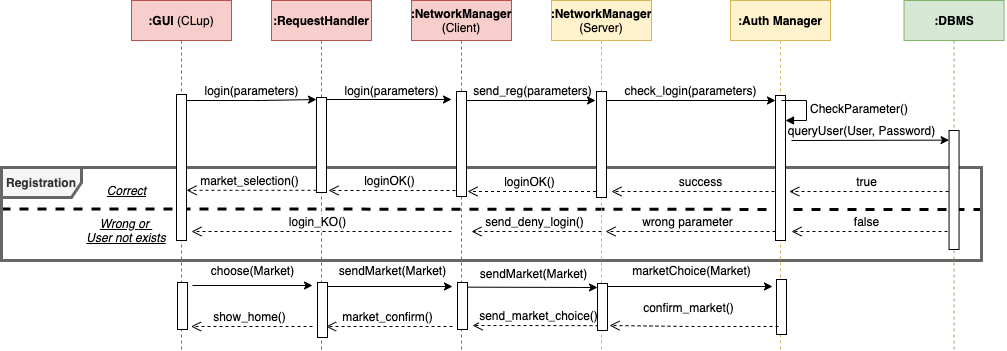
\includegraphics[scale=0.48]{diagrams/LoginSD.png}}
    \caption{The sequence diagram of the CLup's app login.}
\end{figure} 


\begin{figure}[H]
  \label{RegistrationSD}
  \centering
  \makebox[\linewidth]{
  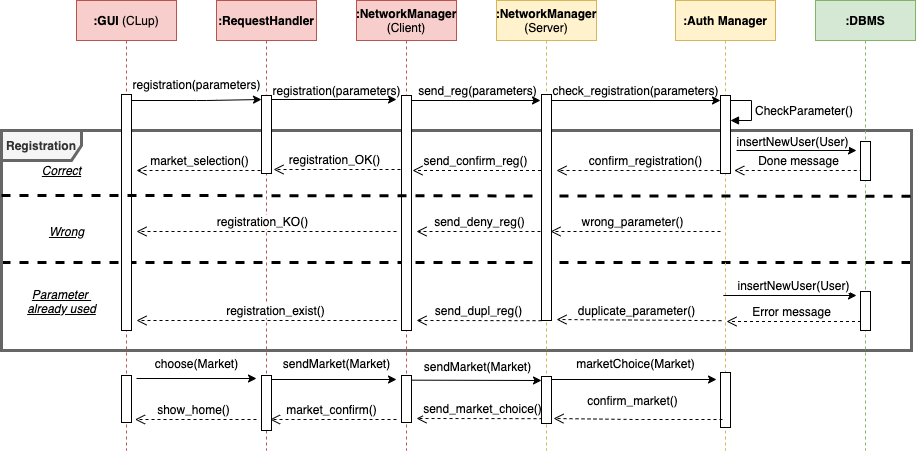
\includegraphics[scale=0.45]{diagrams/RegistrationSD.png}}
    \caption{The sequence diagram of the CLup's app registration.}
\end{figure} 

\subsection{Booking, delay and cancellation}

Any appointment is managed by \textit{Request Handler} which interacts with the \textit{GUI} component to compile an application. Then it's sent to the Server thanks to the \textit{Network Manager} components and processed by the \textit{Reservation Queue} or by the \textit{Visit Schedule}. Any relevant data in our system will be updated, delated, or inserted in our Data base through the RDBMS.


\begin{figure}[H]
  \label{ReservatioSD}
  \centering
  \makebox[\linewidth]{
  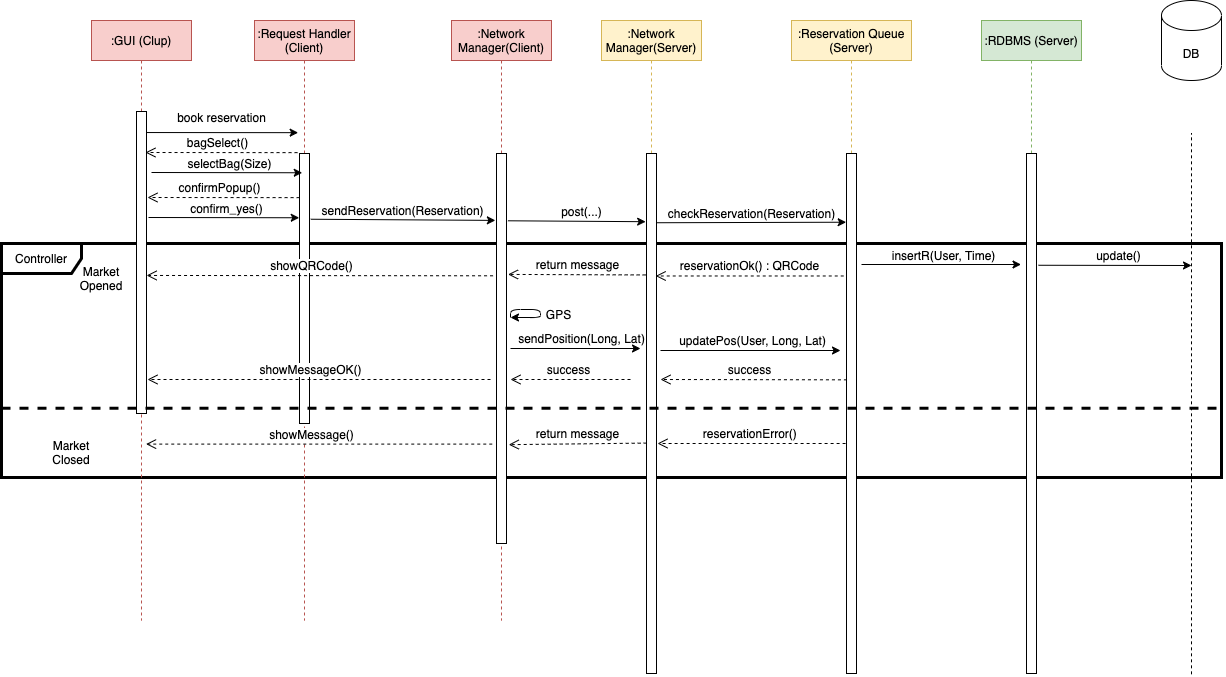
\includegraphics[scale=0.52]{diagrams/ReservationSD.png}}
    \caption{Sequence Diagram of the procedure to be inserted in queue for a Reservation.}
      \label{ReservatioSD}

\end{figure} 


\begin{figure}[H]
  \label{PostponeReservationSD}
  \centering
  \makebox[\linewidth]{
  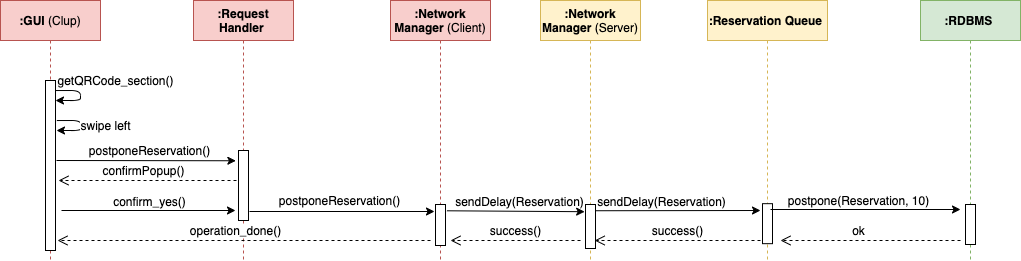
\includegraphics[scale=0.48]{diagrams/PostponeReservationSD.png}}
    \caption{The diagram shows how a generic user postopones his turn in the queue. }
\end{figure} 


\begin{figure}[H]
  \label{VisitSD}
  \centering
  \makebox[\linewidth]{
  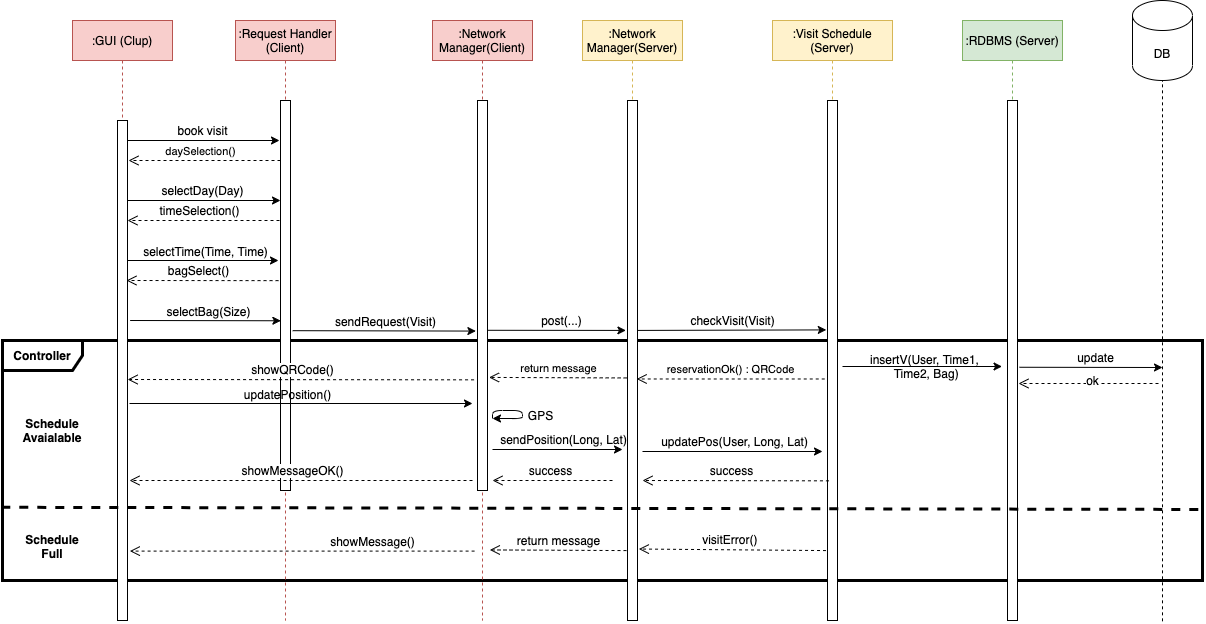
\includegraphics[scale=0.52]{diagrams/VisitSD.png}}
    \caption{Sequence Diagram of the booking procedure of a visit made by an user.}
\end{figure} 




\begin{figure}[H]
  \label{DeleteVisitSD}
  \centering
  \makebox[\linewidth]{
  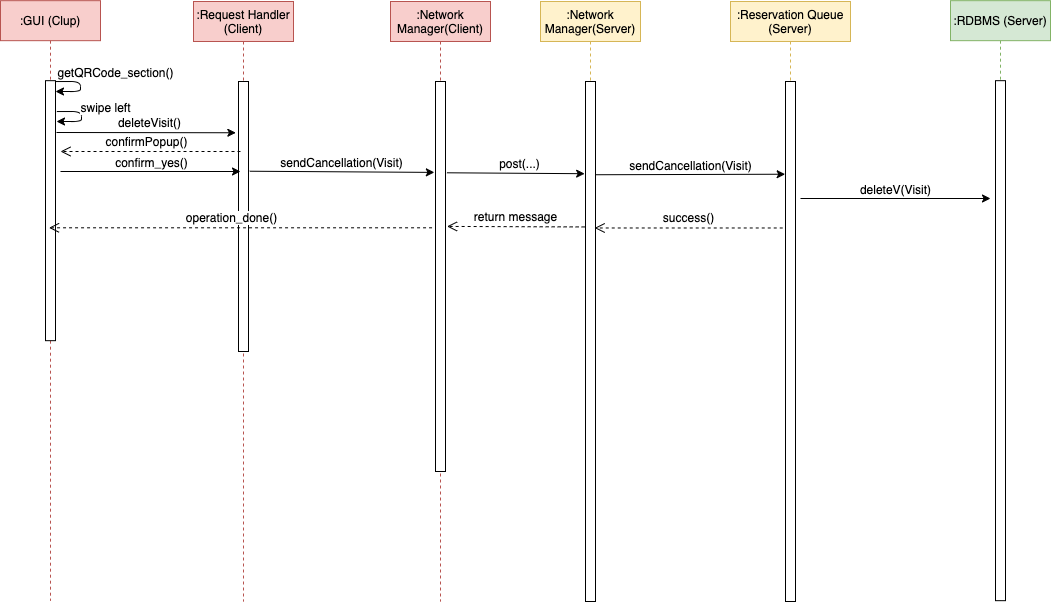
\includegraphics[scale=0.52]{diagrams/DeleteVisitSD.png}}
    \caption{The diagram shows how a generic user deletes his turn from the schedule.}
\end{figure} 


\subsection{Enter and Exit from the market}
This sequence diagram aims to formalize the interaction of the user in the system when he arrives at the entrance of the market and starts his grocery shopping.
An user submit his QRCode through a \textit{QR Reader} which is sent to the Server; then, it will be checked by the \textit{Controller}. Both times of entry and exit will be stored thorugh the RDBMS if the QRCode is valid.

\begin{figure}[H]
  \label{EntryExitSD}
  \centering
  \makebox[\linewidth]{
  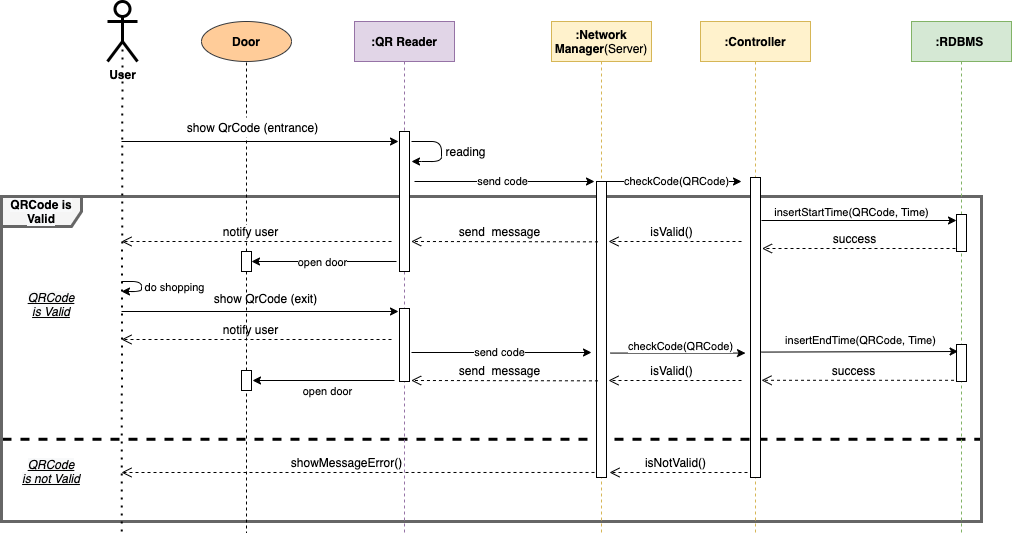
\includegraphics[scale=0.52]{diagrams/EntryExitSD.png}}
    \caption{The SD explain how an user is allowed to enter and exit from the market.}
\end{figure} 

\pagebreak

\subsection{Receptionist}
In this sequence diagram, it's modelled the interaction of the components when a user without a smartphone wants to book a seat in the queue by calling the receptionist of his market. Firstly, while he's speaking on the mobile phone, the receptionist deals with his registration (in the case of a new user), or his recognition (in the case is already registered).
Secondly the procedure to book a reservation will be almost the same in the case described in the SD in figure \ref{ReservatioSD}. The main difference it's the component \textit{Booking Manager}, which differently has higher privileges to retrive and store data in the DB.

\begin{figure}[H]
  \label{MobileUserSD}
  \centering
  \makebox[\linewidth]{
  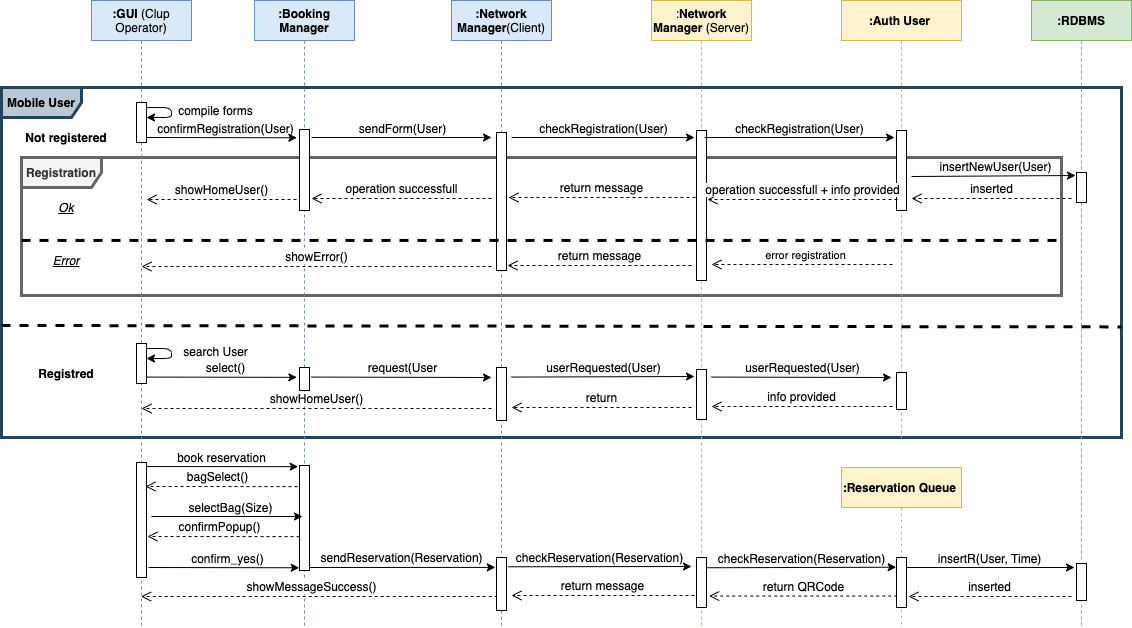
\includegraphics[scale=0.52]{diagrams/MobileUserSD.png}}
    \caption{The SD exaplain how a reservation of mobile user is booked by the receptionist.}
\end{figure} 

\pagebreak

\subsection{Notifications}
This describes how the the application server is working when it has to notify an user about his upcoming turn. At the beginning, the server through the \textit{Controller} checks the schedule by verifiying if can allows a new user in the market. When it could do it, ask for the next user in head of the queue. The first notification is sent in advance to allert the user because it will be almost his turn. While the second will be sent when the turn arrived and the user is allowed to enter. 

\begin{figure}[H]
  \label{NotificationsSD}
  \centering
  \makebox[\linewidth]{
  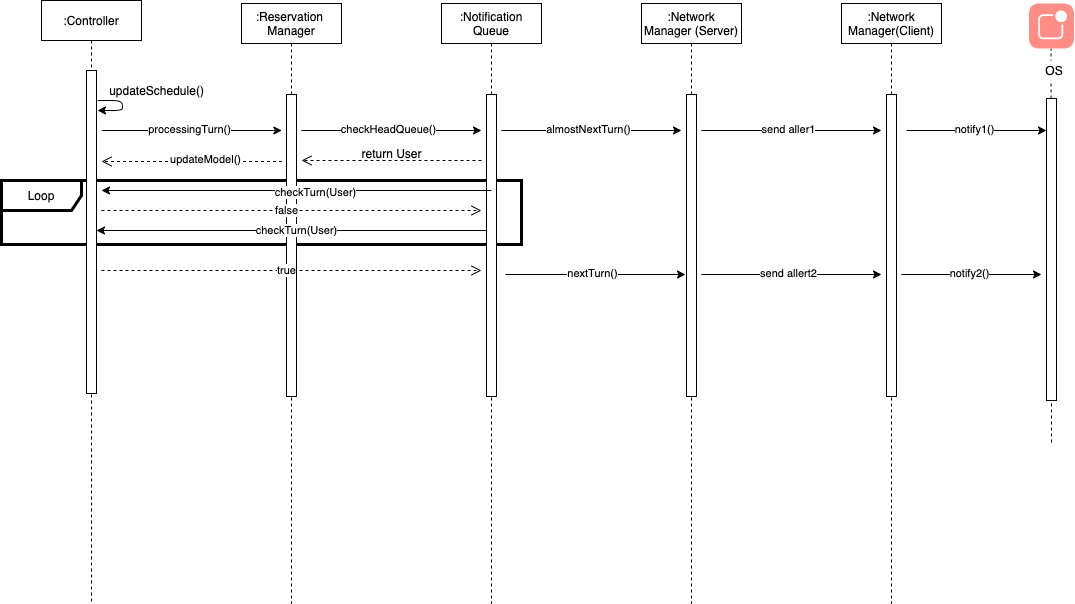
\includegraphics[scale=0.52]{diagrams/NotificationsSD.png}}
    \caption{The sequence diagram exaplain how the system notify for its turn in the queue.}
\end{figure} 

\pagebreak


\section{Component interfaces}
In this section we describe the interfaces needed for the communication between each component. Moreover a list of the main functionalities provided by them is provided.

\begin{itemize}

\item \textbf{Request Handler Interface}: it exposes to the GUI component the following methods:
\begin{itemize}
\item \textit{void selectBag(Size)}: used to confirm the bag size during the booking request (Reservation or Visit);
\item \textit{void confirmYes()} and \textit{void confirmNo()}: used to confirm or not a Reservation;
\item \textit{Boolean bookVisit()} and \textit{Boolean bookReservation()}: used to open a booking request;
\item \textit{Boolean delayReservation()}: used to open a Reservaiton delay;
\item \textit{Boolean cancelReservation()} and \textit{Boolean cancelVisit()}: used to open a Reservation delay;
\end{itemize}

\item \textbf{GUI Interface}: it interacts with the Network Manager and Request Handler components in order to control the \textbf{View} part of our system. 

\item \textbf{Network Interface} (CLup): it interacts with the Request Handler component due to send request to the Application Server;

\item \textbf{Network Interface} (CLup Operator): it interacts with the Booking Manager component in order to send request to the Application Server;


\item \textbf{Scanner Interface}: it interacts with the QR Reader component due to open or close the market's door, depending on the validity of the QRCode;

\item \textbf{Google Maps API Interface}: it interacts with the Network Manager (CLup) component due to locate the own position and the time necessary to reach the market;


\item \textbf{Network Interface} (Server): it interacts with the Controller component in order to:
\begin{itemize}
\item Send responses to the clients;
\item Update, insert, delete and query data of the DB;
\end{itemize}

\item \textbf{Reservation Interface}: it exposes to the Controller component mainly the following methods:
\begin{itemize}
\item \textit{Boolean checkReservation(Reservation)}: it checks and confirms or declines a Reservation request from an User/Receptionist;
\item \textit{Boolean updatePos(User, Long, Lat)}: it updates the current position of an User, in order to estimate his time arriving;
\item \textit{Boolean sendCancellation(Reservation)}: it allows to cancel a Reservation; 
\item \textit{Boolean sendDelay(Reservation)}: it allows to postopone the turn of an User in queue;
\end{itemize}



\item \textbf{Visit Interface}: it exposes to the Controller component mainly the following methods:
\begin{itemize}
\item \textit{Boolean checkVisit(Reservation)}: it checks and confirms or declines a Reservation request from an User/Receptionist;
\item \textit{Boolean updatePos(User, Long, Lat)}: it updates the current position of an User, in order to estimate his time arriving;
\item \textit{Boolean sendCancellation(Reservation)}: it allows to cancel a Reservation; 
\item \textit{Boolean sendDelay(Visit)}: it allows to postopone the turn of an User in queue;
\end{itemize}


\item \textbf{Notification Interface}: it interacts with the Controller component in order to schedule on time notifications that have to be sent to the users;

\item \textbf{Auth User} and \textbf{Auth Rceptionist Interfaces}: they interact with the Controller component in order to check login and registration request from Users and Receptionists;

\item \textbf{DB Interface}: it interacts with the Network Manager component in order to insert, delete and update data in the DB. It exposes to the Network Manager mainly the following methods:
\begin{itemize}
\item \textit{newUser(User, Password, Informations)}: inserts data regarding a new user;
\item \textit{insertReservation(User, Reservation)} and \textit{insertVisit(User, Visit)}: inserts data regarding a new Reservation or Visit;
\item \textit{deleteV(Visit)} and \textit{deleteR(Reservation)}
\item \textit{postpone(Reservation, 10)}: postpone a seat in the queue for a Reservation by 10 minutes;
\item \textit{insertStartTime(QRCode, Time)} and  \textit{insertEndTime(QRCode, Time)}: insert the startTime and endTime for a grocery shopping in the market, associated to its QRCode;
\item \textit{checkCredential(User, Password)}: queries the DB verifying if the user and his credential are correct;
\end{itemize}

\end{itemize}


\section{Selected architectural styles and patterns}
These are the following pattern proposed for a potentially implementation.
\bigskip

\textbf{3 Tiers Architecture} \par
As already mentioned in the section \ref{3-tier} is formed by the Presentation, Application and Data layers. By separating each layer scalability of each component will be improved.
Moreover flexibility is added because of the reduction of development cycle times. Developer in fact can upgrade or replace independently one tier without affecting the others. 
\bigskip

\textbf{Model-View-Controller} \par
MVC is an architectural pattern which can be used to organize the input, processing, and output of an application. It's composed by:
\begin{itemize}
\item \textbf{Model}: it's where the data objects of our business logic is stored;
\item \textbf{Controller}: it's a layer that responds to the users and to changes in the model;
\item \textbf{View}: it represent the user interface;
\end{itemize}

A MVC pattern allows a faster development due to the fact that each layer can be built in parallel to the others. This, also supports an asynchronous technique, which could make our system faster. This is will be very significant for notifications that have to be sent to users in precise moments.
\bigskip
\textbf{Observer} \par
This is a software design pattern usefull for objects which have to notify automatically any state changes to their dependents. We need it due to propagates any changes in our model to its components in a very efficient mannor.

For instance it could be very helpfull for managing a queue variation when it happens (a user cancels his reservation).


\section{Other design decisions}
\textbf{Users Flow in the market} \par
To reach the goal of controlling people into the market and to avoid the queue formation, the Controller component needs an \textbf{algorithm} that allows called users to directly enter without waiting outside. 

This algorithm will be based on:
\begin{itemize}
\item A maximum threshold of people that the market can contain. We call this threshold \textbf{maxThreshold};
\item A tolerance \textbf{margin}, to manage unexpected events and to guarantee that MaxThreshold will not  exceeded in case of slowdowns;
\item A \textbf{data gathering system} that will estimate, basing on users habits, when the system have to notice the next user in queue;
\end{itemize}


The system will be based on informations entered by the users and by statistics of the collected data.
First of all, the shopping size will be requested when the user takes the reservation; in this way it will be possible to predict the maximum shopping time. 
This parameter will be based on a \textbf{user reliability index} that will be estimated by computing how the time of parmanence in the market deviates from his avarage time with the same shopping size. (deviazione standard) \\
For example, the fact that a user selects a "Small" size and goes shopping for 1 hour is less reliable than one that goes shopping for 30 minutes in the shop.
So accordingly to the reliability index, the next user in queue will be noticed with a different timing.

The \textbf{average time} according to shopping size will be estimated on all user reservations and  due to his reliability index.

 

In the case of a new registered user, with no or few reservations, the duration will be estimated exclusively on his average time due to the lack of accuracy of data collected.
In case of usual customer with a low reliability index, the shopping time will be considered according to the client habits without consider clients' \textbf{average shopping time}.

 

The system for each user into the supermarket will monitor the duration of the shopping and when will be near to average, accordingly to the shopping size and reliability index, will call the next user. In order to decide the moment in which a user is called, we consider also the travel time which is how long he takes to reach the shop, based on his position.
If the user will not share own position, the system will use a \textit{standard travel time} (10/15 minutes). In fact, usually the customers go shopping near their home.

 

The system will also consider the visit that will be scheduled during the day in order to manage entrance.
When the system will notice a people overload will have to slow down calls of new customers, in order to never exceeded the entrance maximum number in the market. 
  
\[PeopleInMarket + Margin + PeopleVisit <= MaxThreshold\]

